\section{Issues with the \pa Approach}
\label{sec:motivation}


Despite being inspired by demand paging, the \pa approach is different from it: \textit{\pa implements demand paging in user space whereas conventional demand paging is transparent to applications}. This section elaborates on issues that arise with such an approach.

\subsection{Requires Re-writing the Attention Kernel}
\label{subsec:rewriting}

Conventional implementations of the attention operator assume that the two input tensors K and V (\autoref{eq:attention}) are stored in contiguous memory. By departing from the conventional memory layout, \pa requires an implementation of the attention operator to be modified so as to compute attention scores over non-contiguous \kvcache blocks. Writing correct and performant GPU kernels can be challenging for most programmers~\cite{fa-paged-crash}.


Being a fundamental building block of the transformer architecture, the attention operator has witnessed a tremendous pace of innovation in the systems and ML communities for performance optimizations~\cite{flashattention, flashattention2, flashdecoding, flashdecoding++, flashinfer, h2o2023, flashattnhopper, groupedqueryattention, multiqueryattention, generatinglongsequence2019, longformer, pod-attn-2024}, and this trend is likely to continue. In the \pa model, keeping up with new research requires continued efforts in porting new optimizations to a \pa-aware implementation. Production systems can therefore easily fall behind research, potentially losing performance and competitive advantage. To provide an example,~\autoref{table:eval:decode-attn} shows that the paged kernel of \vllm is already up to $2.8\times$ slower than the \flashattention kernel~\cite{groupedqueryattention}.

\begin{figure}[t!]
    \centering
    %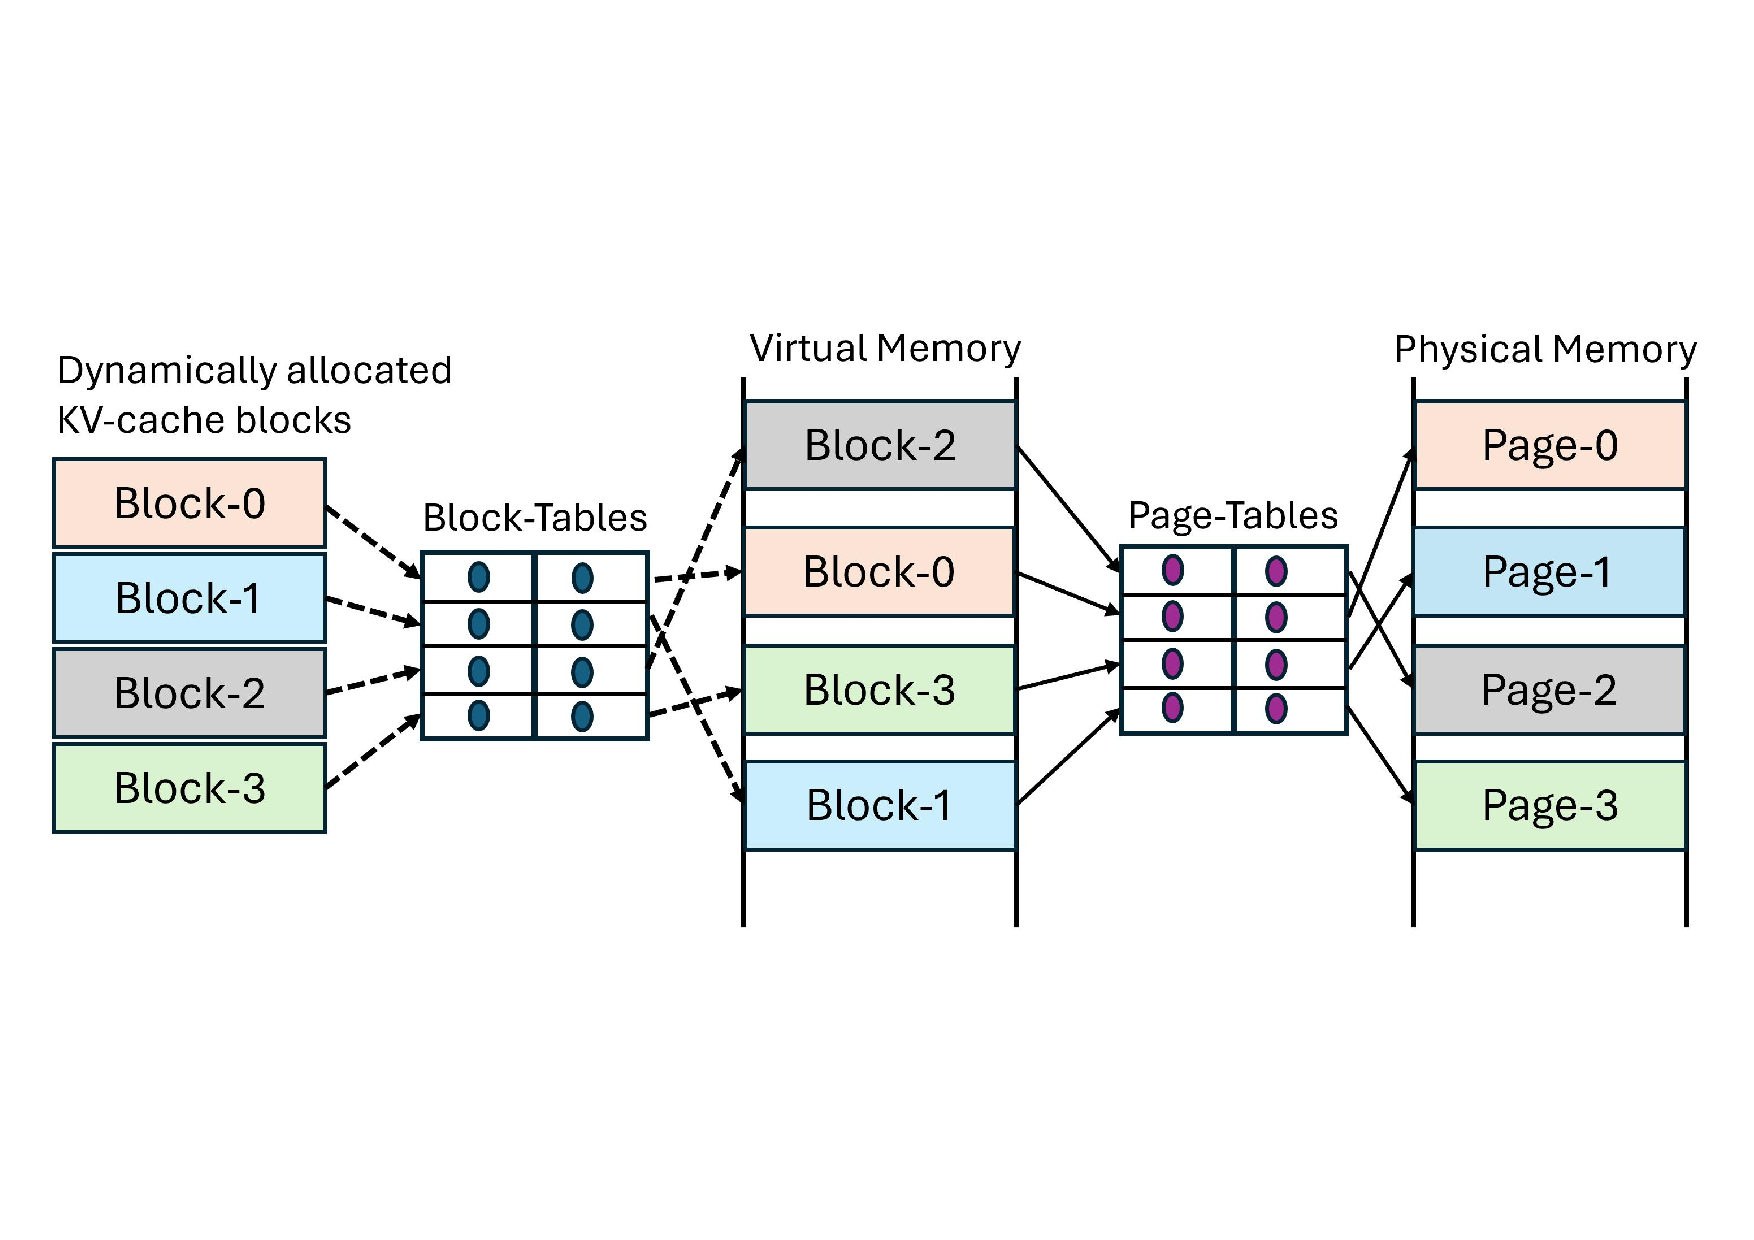
\includegraphics[trim={0 160 0 155}, clip=True, width=0.95\columnwidth]{figures/pa_address_translation2.pdf}
    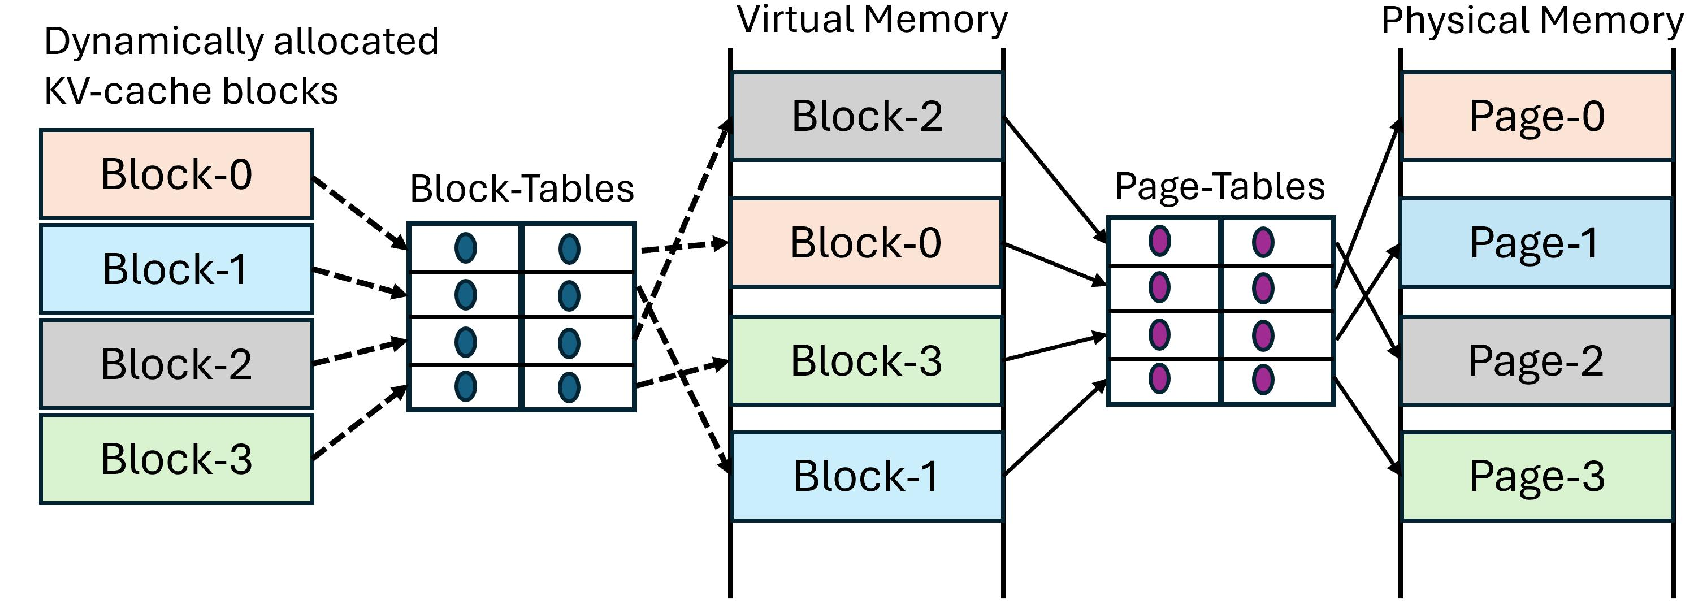
\includegraphics[width=0.95\columnwidth]{figures/pa_address_translation2-cropped.pdf}
    \caption{\pa involves two layers of memory management: one in user space and one in OS kernel space.}
    \label{fig:motivation:pamemlayout}
\end{figure}



\subsection{Adds Redundancy in the Serving Framework}
\label{subsec:blocktable}

\pa makes an LLM serving system responsible for managing the mappings between \kvcache and dynamically allocated memory blocks.
For example, consider a request that allocates four \kvcache blocks over time (left half of~\autoref{fig:motivation:pamemlayout}). These blocks are usually non-contiguous in virtual memory. During the computation of~\autoref{eq:attention}, \pa kernel needs to access all the elements of the four \kvcache blocks. To facilitate this, the serving system needs to track the virtual memory addresses of \kvcache blocks and pass them to the attention kernel at runtime. This approach effectively requires duplicating what the operating system already does for enabling virtual-to-physical address translation (right half in~\autoref{fig:motivation:pamemlayout}).





\subsection{Performance Overhead}
\label{sec:motivation:perfoverhead}


\subsubsection{Runtime overhead on the GPU}
\label{subsec:gpuperfoverhead}
\pa slows down attention computation by adding extra code in the critical path of execution. For example, the \vllm paper acknowledges that the \pa-based implementation was $20-26\%$ slower than the corresponding none-paged FasterTransformer kernel, primarily due to the overhead of looking up Block-Tables and executing extra branches (see Figure 18a in ~\cite{vllmsosp}). In addition, \autoref{fig:motivation:paged-vs-nonpaged} shows that incorporating \pa has also added a significant performance overhead in other state-of-the-art kernel libraries. For example, \pa based prefill kernels of \flashattention and \flashinfer are up to 37\% and 42\% slower than the non-paged kernels in the corresponding libraries. Our analysis reveals that the number of instructions executed in \pa kernels is $7-13\%$ higher than the non-paged kernels. Caching page indices also increases register pressure, causing register spilling.


To highlight another example of difficulty involved in writing an efficient paged kernel, \autoref{fig:eval:vllm:blocksize} shows that the performance of \vllm's paged decode kernel is significantly worse with large block sizes of 64 and 128. Our analysis indicates that this is likely due to L1 cache efficiency: smaller blocks have a higher memory bandwidth utilization due to higher hit rates in the L1 cache.


\begin{figure}[t!]
    \centering
%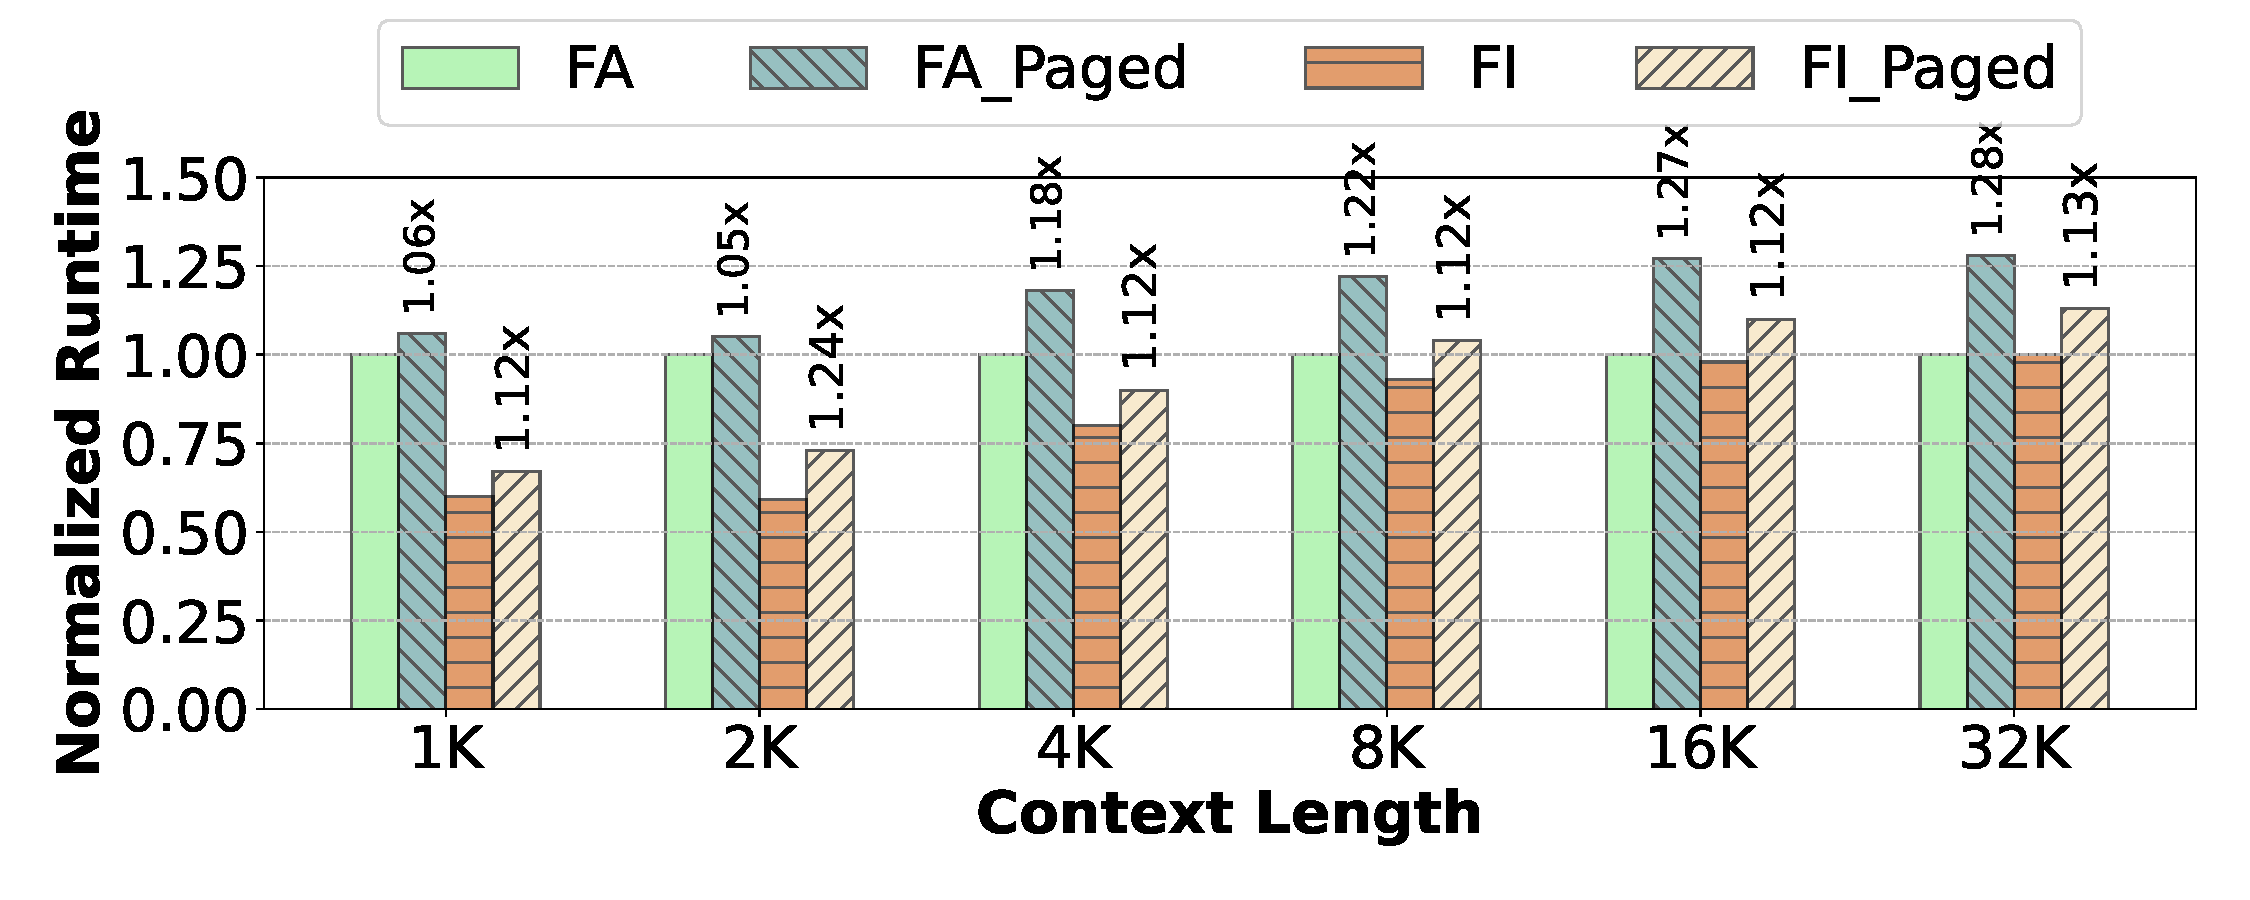
\includegraphics[width=0.95\columnwidth]{graphs/analysis_paged/analysis_paged.pdf}
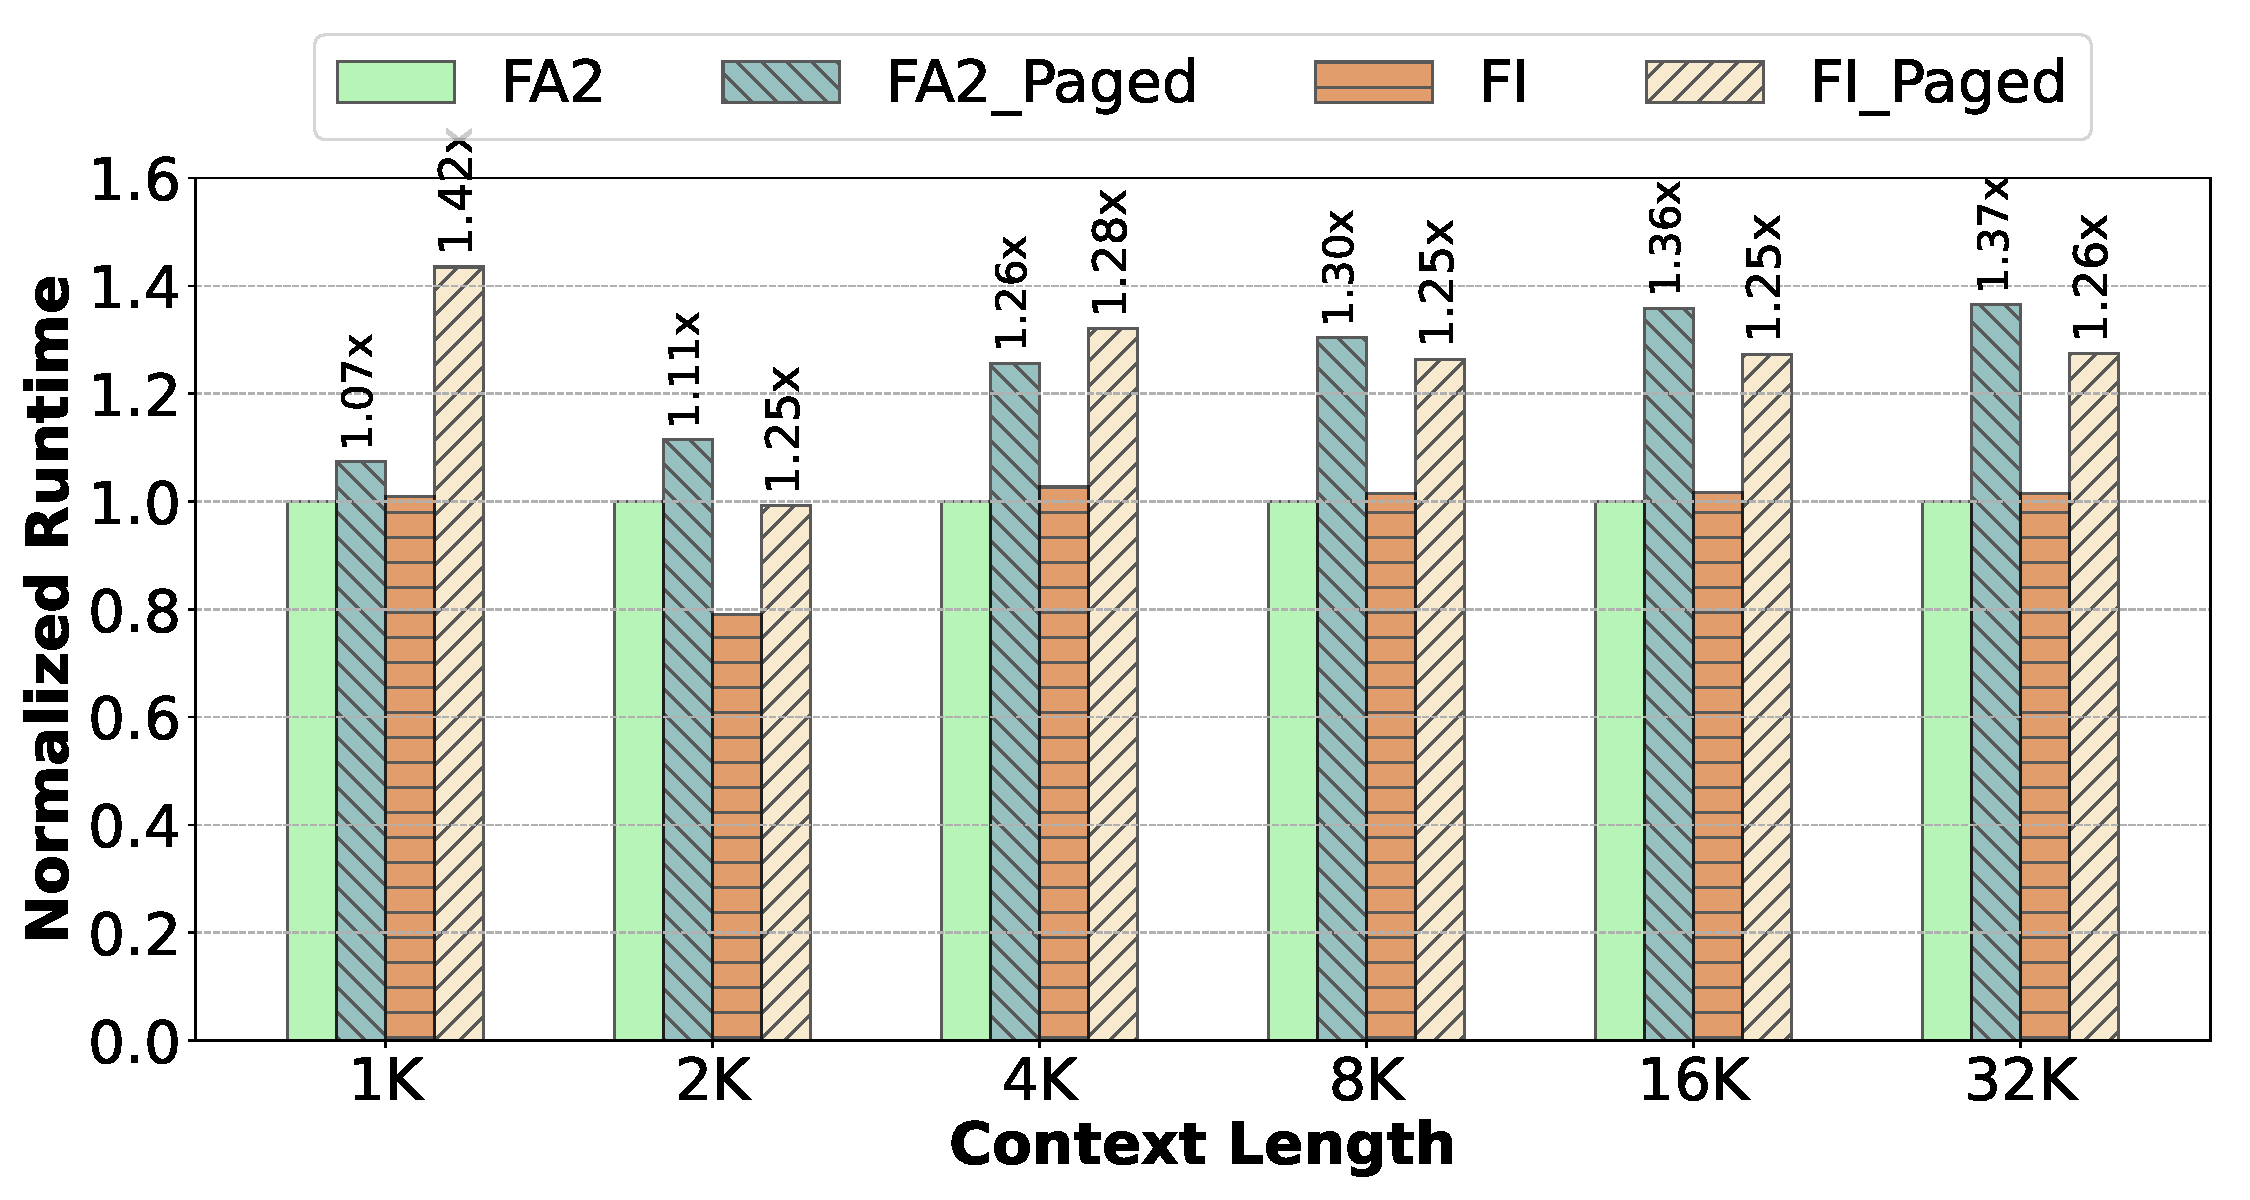
\includegraphics[width=0.9\columnwidth]{graphs/figure_2.pdf}
    \caption{Overhead of \pa in prefill kernels (model: \llamasmall, one A100 GPU). Numbers on top show overhead over the corresponding non-paged implementation of \flashattention (FA2) and \flashinfer (FI).}
    \label{fig:motivation:paged-vs-nonpaged}
\end{figure}

\begin{figure}[t!]
    \centering
    %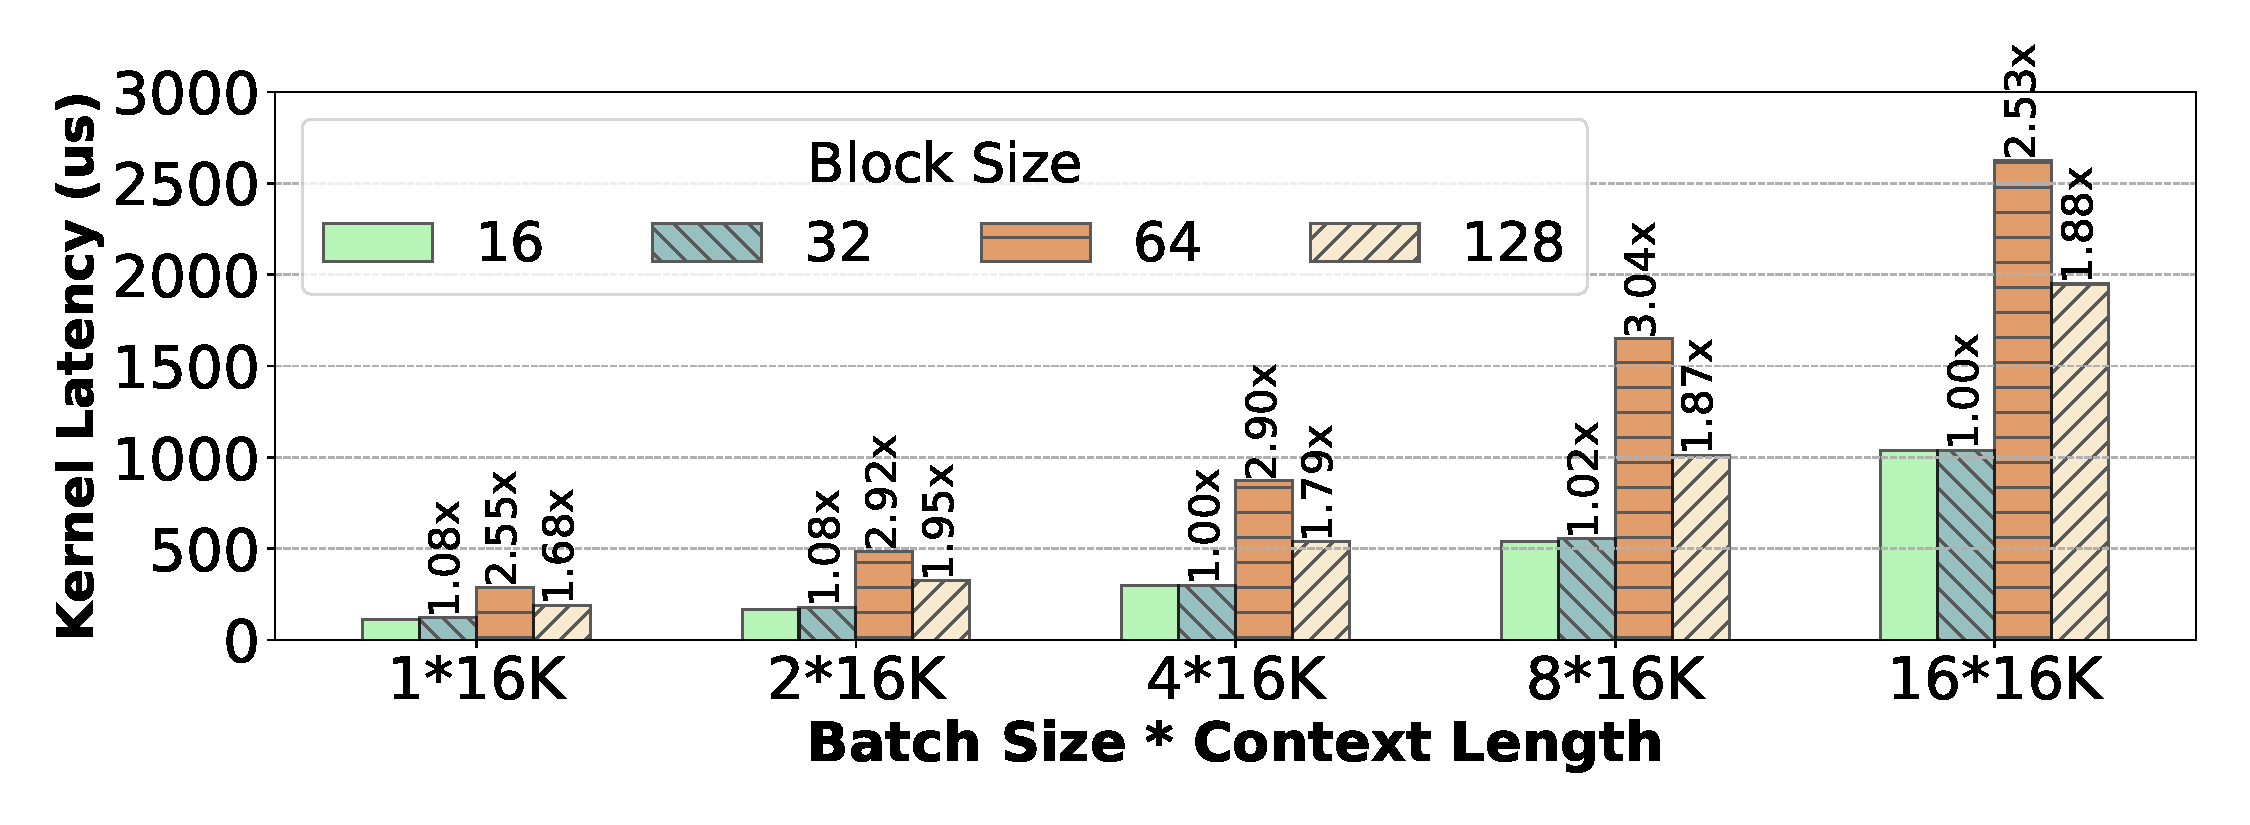
\includegraphics[trim={0 30 0 0}, clip=True, width=0.99\columnwidth]{graphs/analysis_vllm_blocksize/vllm_block_size.pdf}
    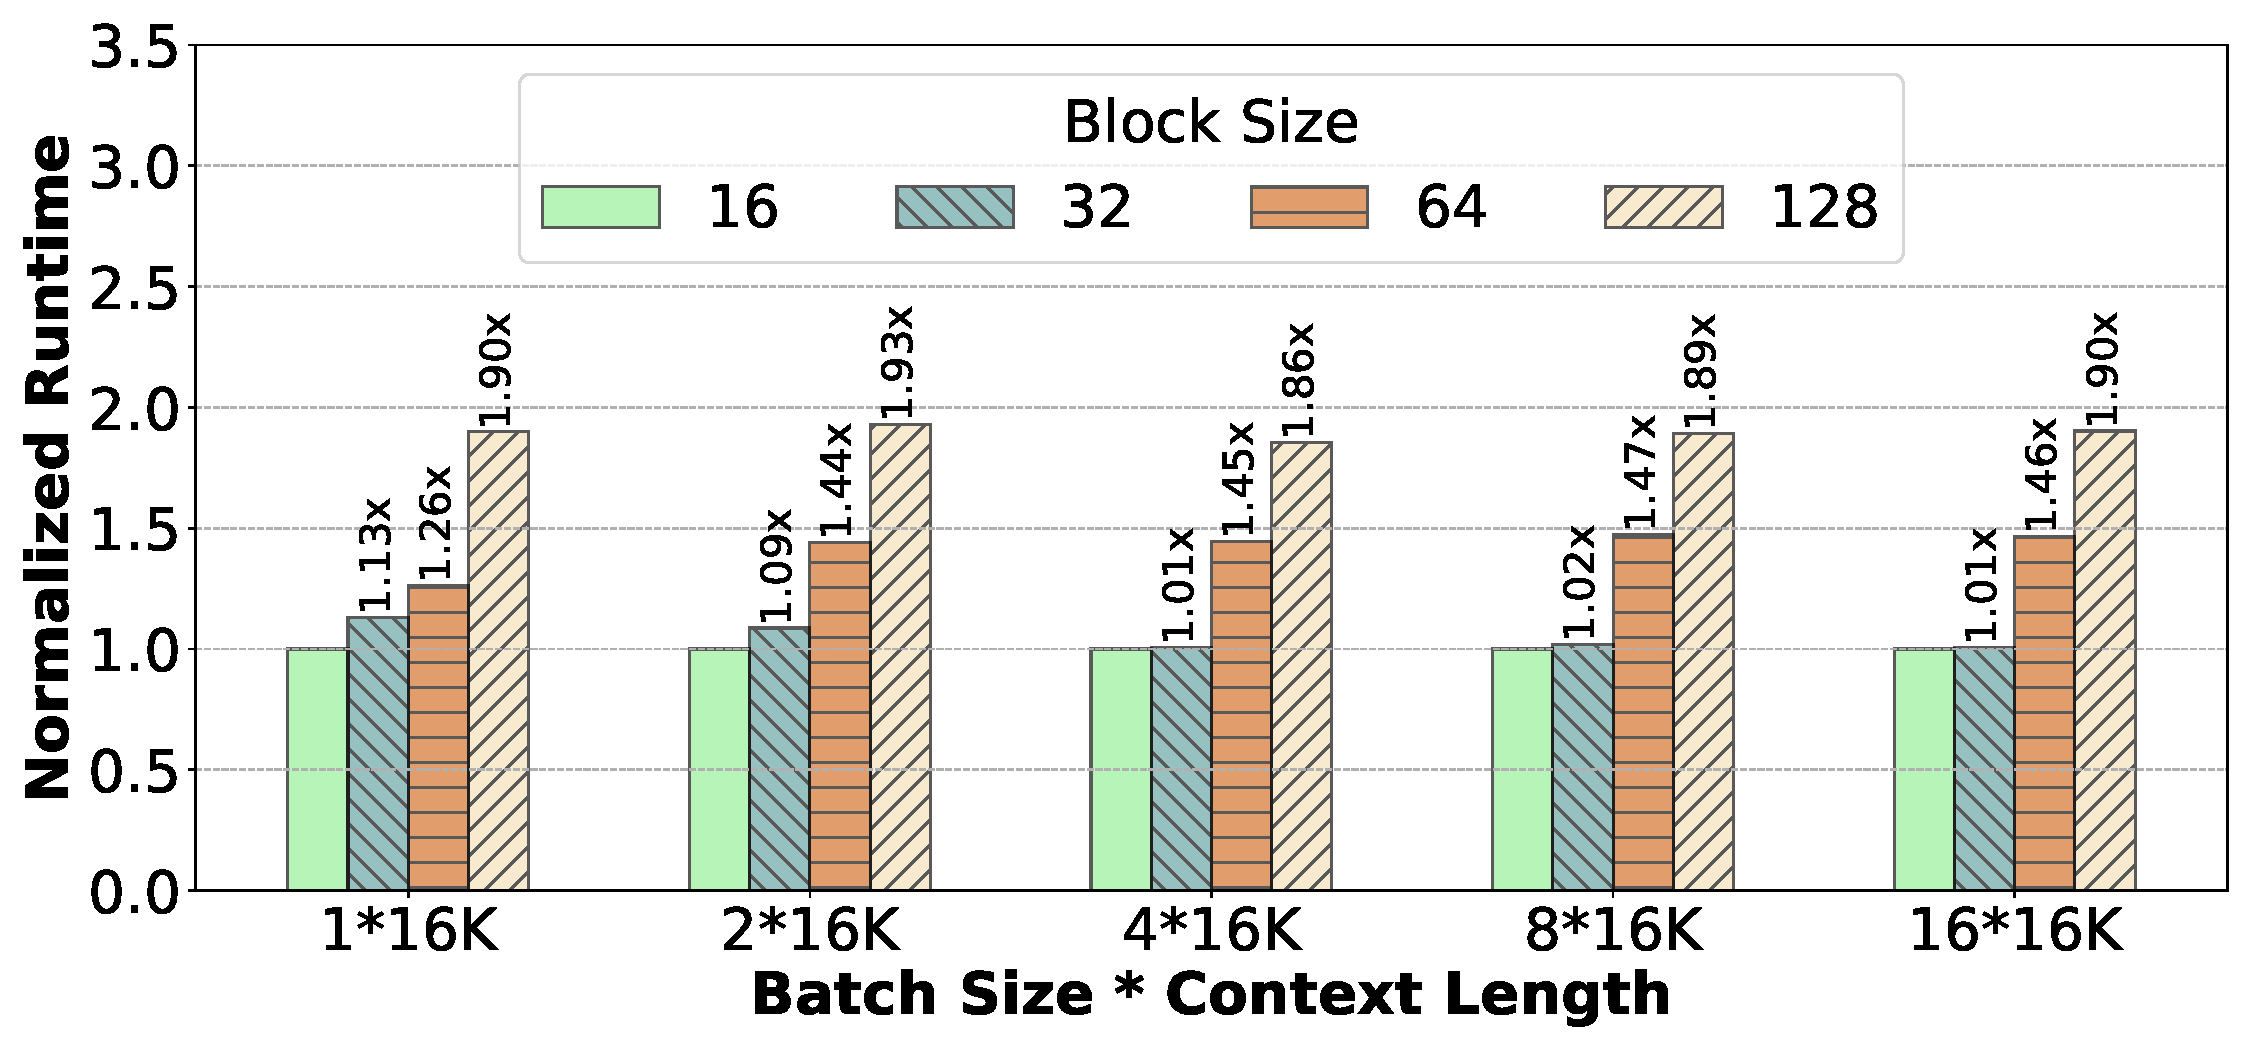
\includegraphics[width=0.9\columnwidth]{graphs/figure_3.pdf}
    \caption{Latency of \vllm's paged decode kernel is sensitive to block size (model: \llamasmall, one A100 GPU).}
    \label{fig:eval:vllm:blocksize}
\end{figure}


\subsubsection{Runtime overhead on the CPU}
\label{subsec:cpuperfoverhead}
Implementing an additional memory manager can add performance issues in the CPU runtime of the serving system. We refer to a few real-world examples and our own observations on \vllm to corroborate this argument.


To enable \pa, a serving system needs to supply Block-Tables to the attention kernel. In \vllm, the latency of preparing a Block-Table depends on batch composition and grows  proportional to \texttt{max\_num\_blocks} $\times$ \texttt{batch\_size} where \texttt{max\_num\_blocks} refers to the number of \kvcache blocks in the longest request of the batch. This is because \vllm manages a Block-Table as a 2D tensor and aligns the number of \kvcache blocks in each request by padding unoccupied slots with zeros. If a batch contains a few long and many short requests, such padding results in a significant overhead. In our earlier experiments, we observed that Block-Table preparation in \vllm was contributing 30\% latency in decode iterations. While a recent fix~\cite{vllm-blocktable-issue} has mitigated some of this overhead, we find that it can still be as high as $10\%$. High overhead of \pa has also been found in TensorRT-LLM, degrading throughput by 11\%~\cite{tensorrt-perf-decay}. This issue was attributed to the Python runtime of TensorRT-LLM and moving to a C++ runtime can mitigate the CPU overhead. However, doing so requires non-trivial programming effort.



 
Overall, this section shows that \pa adds a significant programming burden while also being inefficient. In \sysname, we propose a more principled approach to  dynamic \kvcache memory management. However, before delving into \sysname, we first highlight some of the fundamental characteristics of LLM serving workloads from a memory management perspective.








